%%%%%%%%%%%%%%%%%%%%%%%%%%%%%%%%%%%%%%%%%
% Masters/Doctoral Thesis 
% LaTeX Template
% Version 2.5 (27/8/17)
%
% This template was downloaded from:
% http://www.LaTeXTemplates.com
%
% Version 2.x major modifications by:
% Vel (vel@latextemplates.com)
%
% This template is based on a template by:
% Steve Gunn (http://users.ecs.soton.ac.uk/srg/softwaretools/document/templates/)
% Sunil Patel (http://www.sunilpatel.co.uk/thesis-template/)
%
% Template license:
% CC BY-NC-SA 3.0 (http://creativecommons.org/licenses/by-nc-sa/3.0/)
%
%%%%%%%%%%%%%%%%%%%%%%%%%%%%%%%%%%%%%%%%%


%----------------------------------------------------------------------------------------
%	PACKAGES AND OTHER DOCUMENT CONFIGURATIONS
%----------------------------------------------------------------------------------------

\documentclass[
11pt, % The default document font size, options: 10pt, 11pt, 12pt
%oneside, % Two side (alternating margins) for binding by default, uncomment to switch to one side
% serbian, % ngerman for German
serbian,
singlespacing, % Single line spacing, alternatives: onehalfspacing or doublespacing
%draft, % Uncomment to enable draft mode (no pictures, no links, overfull hboxes indicated)
%nolistspacing, % If the document is onehalfspacing or doublespacing, uncomment this to set spacing in lists to single
%liststotoc, % Uncomment to add the list of figures/tables/etc to the table of contents
%toctotoc, % Uncomment to add the main table of contents to the table of contents
%parskip, % Uncomment to add space between paragraphs
% nohyperref, % Uncomment to not load the hyperref package
headsepline, % Uncomment to get a line under the header
%chapterinoneline, % Uncomment to place the chapter title next to the number on one line
%consistentlayout, % Uncomment to change the layout of the declaration, abstract and acknowledgements pages to match the default layout
]{MastersDoctoralThesis} % The class file specifying the document structure

\usepackage[utf8]{inputenc} % Required for inputting international characters
\usepackage[T1]{fontenc} % Output font encoding for international characters

%\usepackage{mathpazo} % Use the Palatino font by default
\usepackage{amsmath}
% dužine

\usepackage{listings}                                                           
\usepackage{color}

\definecolor{mygreen}{rgb}{0,0.6,0}
\definecolor{mygray}{rgb}{0.5,0.5,0.5}
\definecolor{mymauve}{rgb}{0.58,0,0.82}

                                                                                

% \usepackage[backend=bibtex,style=authoryear,natbib=true]{biblatex} % Use the bibtex backend with the authoryear citation style (which resembles APA)
\usepackage[
  backend=bibtex
  , natbib=true
  , citestyle=numeric
  , bibstyle=numeric
  , sorting=none
  , maxbibnames=99
]{biblatex} % Use the bibtex backend with the authoryear citation style (which resembles APA)


\addbibresource{bib/main.bib} % The filename of the bibliography


% \usepackage[autostyle=true]{csquotes} % Required to generate language-dependent quotes in the bibliography

%----------------------------------------------------------------------------------------
%	MARGIN SETTINGS
%----------------------------------------------------------------------------------------

\geometry{
	paper=a4paper, % Change to letterpaper for US letter
	% inner=3.15cm, % Inner margin
	% outer=3.15cm, % Outer margin
	% bindingoffset=0cm, % Binding offset
	inner=2.5cm, % Inner margin
	outer=3.8cm, % Outer margin
	bindingoffset=.5cm, % Binding offset
	top=1.5cm, % Top margin
	bottom=1.5cm, % Bottom margin
  % showframe, % Uncomment to show how the type block is set on the page
}

%----------------------------------------------------------------------------------------
%	THESIS INFORMATION
%----------------------------------------------------------------------------------------

\thesistitle{Razvoj metaprediktora za utvrđivanje neuređenosti proteina} % Your thesis title, this is used in the title and abstract, print it elsewhere with \ttitle

\supervisor{Jovana \textsc{Kovačević}} % Your supervisor's name, this is used in the title page, print it elsewhere with \supname
\examiner{} % Your examiner's name, this is not currently used anywhere in the template, print it elsewhere with \examname
\degree{Master informatičar} % Your degree name, this is used in the title page and abstract, print it elsewhere with \degreename
\author{Una \textsc{Stanković}} % Your name, this is used in the title page and abstract, print it elsewhere with \authorname
\addresses{https://www.linkedin.com/in/una-stankovic-443a35137/} % Your address, this is not currently used anywhere in the template, print it elsewhere with \addressname

\subject{Bioinformatika} % Your subject area, this is not currently used anywhere in the template, print it elsewhere with \subjectname
\keywords{} % Keywords for your thesis, this is not currently used anywhere in the template, print it elsewhere with \keywordnames
\university{\href{http://www.bg.ac.rs}{Univerzitet u Beogradu}} % Your university's name and URL, this is used in the title page and abstract, print it elsewhere with \univname
\department{\href{http://www.racunarstvo.matf.bg.ac.rs/}{Katedra za Računarstvo i informatiku}} % Your department's name and URL, this is used in the title page and abstract, print it elsewhere with \deptname
\group{.} % Your research group's name and URL, this is used in the title page, print it elsewhere with \groupname
% \group{\href{http://researchgroup.university.com}{Research Group Name}} % Your research group's name and URL, this is used in the title page, print it elsewhere with \groupname
\faculty{\href{http://matf.bg.ac.rs}{Matematički fakultet}} % Your faculty's name and URL, this is used in the title page and abstract, print it elsewhere with \facname

\AtBeginDocument{
\hypersetup{pdftitle=\ttitle} % Set the PDF's title to your title
\hypersetup{pdfauthor=\authorname} % Set the PDF's author to your name
\hypersetup{pdfkeywords=\keywordnames} % Set the PDF's keywords to your keywords
}

\begin{document}

\frontmatter % Use roman page numbering style (i, ii, iii, iv...) for the pre-content pages

\pagestyle{plain} % Default to the plain heading style until the thesis style is called for the body content

%----------------------------------------------------------------------------------------
%	TITLE PAGE
%----------------------------------------------------------------------------------------

\begin{titlepage}
\begin{center}

\vspace*{.06\textheight}
{\scshape\LARGE \univname\par} % University name
{\scshape\LARGE \facname\par} % University name
\vspace{1.5cm}
\textsc{\Large Master Rad}\\[0.5cm] % Thesis type

\HRule \\[0.4cm] % Horizontal line
{\huge \bfseries \ttitle\par}\vspace{0.4cm} % Thesis title
\HRule \\[1.5cm] % Horizontal line
 
\begin{minipage}[t]{0.4\textwidth}
\begin{flushleft} \large
\emph{Autor:}\\
\href{https://www.linkedin.com/in/una-stankovic-443a35137/}{\authorname} % Author name - remove the \href bracket to remove the link
\end{flushleft}
\end{minipage}
\begin{minipage}[t]{0.4\textwidth}
\begin{flushright} \large
\emph{Mentor:} \\
\href{http://poincare.matf.bg.ac.rs/~jovana/}{\supname} % Supervisor name - remove the \href bracket to remove the link  
\end{flushright}
\end{minipage}\\[2cm]
 
\vfill

% \large \textit{A thesis submitted in fulfillment of the requirements\\ for the degree of \degreename}\\[0.3cm] % University requirement text
% \textit{in the}\\[0.4cm]
% \groupname\\\deptname\\[2cm] % Research group name and department name

{\scshape\LARGE Članovi komsije:\par}\vspace{0.2cm} % University name
dr Jovana Kovačević \\
prof. dr Gordana Pavlović-Lažetić  \\
dr Nina Radojičić \\

 
\vfill

\vspace{1cm}
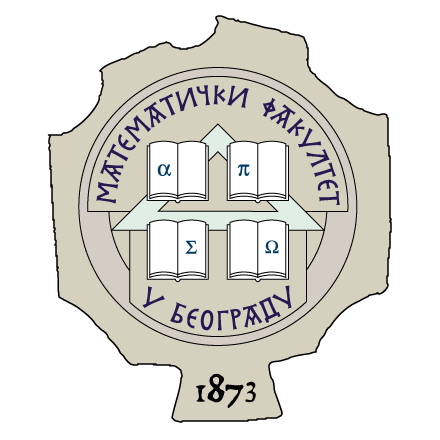
\includegraphics[scale=0.25]{Logo}\\ % University/department logo - uncomment to place it
\vspace{0.5cm}
{\large Beograd, 2018}\\ % Date
 
\vfill
\end{center}
\end{titlepage}

%----------------------------------------------------------------------------------------
%	DECLARATION PAGE
%----------------------------------------------------------------------------------------

% \begin{declaration}
% \addchaptertocentry{\authorshipname} % Add the declaration to the table of contents
% \noindent I, \authorname, declare that this thesis titled, \enquote{\ttitle} and the work presented in it are my own. I confirm that:
%
% \begin{itemize} 
% \item This work was done wholly or mainly while in candidature for a research degree at this University.
% \item Where any part of this thesis has previously been submitted for a degree or any other qualification at this University or any other institution, this has been clearly stated.
% \item Where I have consulted the published work of others, this is always clearly attributed.
% \item Where I have quoted from the work of others, the source is always given. With the exception of such quotations, this thesis is entirely my own work.
% \item I have acknowledged all main sources of help.
% \item Where the thesis is based on work done by myself jointly with others, I have made clear exactly what was done by others and what I have contributed myself.\\
% \end{itemize}
%  
% \noindent Signed:\\
% \rule[0.5em]{25em}{0.5pt} % This prints a line for the signature
%  
% \noindent Date:\\
% \rule[0.5em]{25em}{0.5pt} % This prints a line to write the date
% \end{declaration}
%
% \cleardoublepage

%----------------------------------------------------------------------------------------
%	QUOTATION PAGE
%----------------------------------------------------------------------------------------

% \vspace*{0.2\textheight}
%
% \noindent\enquote{\itshape Thanks to my solid academic training, today I can write hundreds of words on virtually any topic without possessing a shred of information, which is how I got a good job in journalism.}\bigbreak
%
% \hfill Dave Barry

%----------------------------------------------------------------------------------------
%	ABSTRACT PAGE
%----------------------------------------------------------------------------------------

% definišemo korisne komande
\newcommand{\en}[1]{(engl. \textit{#1})}
\newcommand{\lat}[1]{(latin. \textit{#1})}
\newcommand{\keyword}[1]{\textbf{#1}}
\newcommand{\ikeyword}[1]{\textit{\textbf{#1}}}
\newcommand{\tabhead}[1]{\textbf{#1}}
\newcommand{\code}[1]{\texttt{#1}}
\newcommand{\file}[1]{\texttt{\bfseries#1}}
\newcommand{\option}[1]{\texttt{\itshape#1}}


\newcommand{\uniprot}{\textit{UniProt} }
\newcommand{\uniprotkb}{\textit{UniProtKB} }
\newcommand{\swissprot}{\textit{Swiss-Prot} }
\newcommand{\trembl}{\textit{TrEMBL} }

\newcommand{\kw}[1]{\textbf{\textit{KW: #1}}}
\newcommand{\mf}[1]{\textbf{\textit{MF: #1}}}

\newtheorem{definicija}{Definicija}

\begin{abstract}
\addchaptertocentry{\abstractname} % Add the abstract to the table of contents
% The Thesis Abstract is written here (and usually kept to just this page). The page is kept centered vertically so can expand into the blank space above the title too\ldots

Coming soon!

\end{abstract}

%----------------------------------------------------------------------------------------
%	ACKNOWLEDGEMENTS
%----------------------------------------------------------------------------------------

\begin{acknowledgements}
\addchaptertocentry{\acknowledgementname} % Add the acknowledgements to the table of contents


\end{acknowledgements}
%
%----------------------------------------------------------------------------------------
%	LIST OF CONTENTS/FIGURES/TABLES PAGES
%----------------------------------------------------------------------------------------

\tableofcontents % Prints the main table of contents

% \listoffigures % Prints the list of figures

% \listoftables % Prints the list of tables

%----------------------------------------------------------------------------------------
%	ABBREVIATIONS
%----------------------------------------------------------------------------------------

% \begin{abbreviations}{ll} % Include a list of abbreviations (a table of two columns)
%
% \textbf{LAH} & \textbf{L}ist \textbf{A}bbreviations \textbf{H}ere\\
% \textbf{WSF} & \textbf{W}hat (it) \textbf{S}tands \textbf{F}or\\
%
% \end{abbreviations}

%----------------------------------------------------------------------------------------
%	PHYSICAL CONSTANTS/OTHER DEFINITIONS
%----------------------------------------------------------------------------------------

% \begin{constants}{lr@{${}={}$}l} % The list of physical constants is a three column table
%
% % The \SI{}{} command is provided by the siunitx package, see its documentation for instructions on how to use it
%
% Speed of Light & $c_{0}$ & \SI{2.99792458e8}{\meter\per\second} (exact)\\
% %Constant Name & $Symbol$ & $Constant Value$ with units\\
%
% \end{constants}

%----------------------------------------------------------------------------------------
%	SYMBOLS
%----------------------------------------------------------------------------------------

% \begin{symbols}{lll} % Include a list of Symbols (a three column table)
%
% $a$ & distance & \si{\meter} \\
% $P$ & power & \si{\watt} (\si{\joule\per\second}) \\
% %Symbol & Name & Unit \\
%
% \addlinespace % Gap to separate the Roman symbols from the Greek
%
% $\omega$ & angular frequency & \si{\radian} \\
%
% \end{symbols}

%----------------------------------------------------------------------------------------
%	DEDICATION
%----------------------------------------------------------------------------------------

 \dedicatory{Tati, mami i Olgi\ldots} 

%----------------------------------------------------------------------------------------
%	THESIS CONTENT - CHAPTERS
%----------------------------------------------------------------------------------------

\mainmatter % Begin numeric (1,2,3...) page numbering

\pagestyle{thesis} % Return the page headers back to the "thesis" style



% Include the chapters of the thesis as separate files from the Chapters folder
% Uncomment the lines as you write the chapters

% Chapter 1

\chapter{Uvod} % Main chapter title

\label{Chapter1} % For referencing the chapter elsewhere, use \ref{Chapter1} 

%This is only a temporary version of introduction based on an application submitted to the committee

Proteini su biološki makromolekuli neophodni za izgradnju i pravilno funkcionisanje ćelija i igraju mnogobrojne uloge u različitim procesima koji se odvijaju unutar organizma. Struktura proteina zavisi od redosleda aminokiselina i utiče na njegovu funckiju. Primarna struktura podrazumeva niz aminokiselina koje učestvuju u izgradnji proteina, dok se sekundarna odnosi na oblik koji protein zauzima u prostoru (spirala ili traka). Proteine sa nestabilnom sekundarnom strukturom nazivamo neuređenim. Pored značajne uloge u obavljanju brojnih bioloških funkcija, otkriveno je i postojanje veze između ovih proteina i razvoja neizlečivih bolesti i zbog toga su oni u fokusu bioinformatičke zajednice.\\\\

Neuređenost proteina se utvrđuje eksperimentalno, laboratorijskim analizama, ili uz pomoć prediktora za automatsko predviđanje neuređenosti proteina. Laboratorijske analize spadaju u spore, veoma skupe metode, koje ne mogu da odgovore na potrebe akademske zajednice i industrije. Iz tog razloga, poslednjih godina, došlo je do razvoja velikog broja alata za automatsko predviđanje neuređenosti proteina. Zbog velike brojnosti ovih alata, razvijaju se metaprediktori koji predstavljaju njihove kombinacije. Specifičan cilj ovog master rada je razvoj jednog metaprediktora za određivanje neuređenosti proteina koji bi konsenzusom objedinio rezultate najnovijih prediktivnih alata na osnovu metodologije na kojoj su zasnovani. Alat će biti testiran na skupu proteina sa eksperimentalno utvrđenom neuređenošću DisProt (eng.~{\em DisProt}).
% =================================================================================================
\chapter{Biološke osnove} % Main chapter title
\label{bioloskeosnove} % For referencing the chapter elsewhere, use \ref{Chapter1} 
% =================================================================================================

U ovoj sekciji biće ukratko predstavljene biološke osnove neophodne za razumevanje rada i motivacije koja stoji iza određenih njegovih elemenata.
Najpre, biće opisano šta su proteini, koje su njihove osnovne funkcije i kakva im je struktura. Potom, biće opisana svaka od struktura ponaosob, uz priložen grafički prikaz istih. Na kraju, posebno će biti opisani neuređeni proteini, njihova uloga i uzroci koji mogu dovesti do njihove pojave. 

% -------------------------------------------------------------------------------------------------
\section{Proteini}
\label{sec:proteini}
% -------------------------------------------------------------------------------------------------

Proteini (grč.~{\em protos} - $"$zauzimam prvo mesto$"$) su biološki makromolekuli neophodni za izgradnju i pravilno funkcionisanje ćelija, i igraju mnogobrojne uloge u različitim procesima koji se odvijaju unutar organizma. Oni su najvažniji sastojak žive materije i utiču na brojnost i raznolikost živih bića. Specifičnost proteina je tolika da svaka biljna i životinjska vrsta ima svoje proteine, a kod viših organizama oni se razlikuju i na individualnom nivou. Broj proteina u živim bićima je ogroman, a kao primer uzmimo $E. coli$ sa $3000$ i čoveka sa $5$ miliona proteina~\cite{spasic}. \\\\
Proteini i peptidi su izgrađeni od $22$\footnote{Neki proteini u svom sastavu mogu da imaju $22$ različite aminokiseline. Pored $20$ “standardnih” aminokiselina,
postoje i $2$ “nestandardne” i to su Selenocistein (eng.~{\em Selenocysteine}, simboli $Sec$, $U$) i Pirolizin (eng.~{\em Pyrrolysine},
simboli $Pyl$, $O$). Ove dve aminokiseline se ređe javljaju~\cite{MarijaJ}.} $L-aminokiseline$ \footnote{$L-aminokiseline$ su one sa levom prostornom konfiguracijom, analogno, postoje i $D-aminokiseline$, sa desnom} koje se javljaju u prirodi i povezani su peptidnim vezama~\cite{biopathways}, koje nastaju između $\alpha$-karboksilne grupe jedne aminokiseline i $\alpha$-amino grupe druge aminokiseline, pri čemu se oslobađa molekul vode~\cite{MarijaJ}. Ovim postupkom nastaje nerazgranati polipeptidni lanac izgrađen od glavnog lanca, koji se pravilno ponavlja, i međusobno različitih ogranaka. $"$Standardna$"$ grupa aminokiselina se može podeliti na esecijalne i
neesecijalne, čiji spisak se može videti u tabeli \ref{table:1}~\cite{MarijaJ}. 
\begin{table}[h!]
\centering
	\begin{tabular}{||c c||} 
	\hline 
	Esencijalne & Neesencijalne \\ [0.5ex] 
	\hline\hline
	Arginin & Alanin \\ 
	\hline
	Histidin & Asparagin \\
	\hline
	Leucin & Asparaginska kiselina\\
	\hline
	Izoleucin & Cistein \\
	\hline
	Lizin & Glutaminska kiselina \\ [1ex] 
	\hline
	Metionin & Glutamin \\ [1ex] 
	\hline
	Fenilalanin & Glicin \\ [1ex] 
	\hline
	Treonin & Prolin \\ [1ex] 
	\hline
	Triptofan & Serin \\ [1ex] 
	\hline
	Valin & Tirozin \\ [1ex] 
	\hline
	\end{tabular}
\caption{Spisak esencijalnih i neesencijalnih aminokiselina}
\label{table:1}
\end{table}
Poznavanje i razumevanje funkcija proteina je esencijalno u istraživanju bilo kog biološkog procesa, sa posebnim naglaskom na oboljenja ljudi, s obzirom da
se mnoga od njih mogu pojaviti zbog funkcionalnih mutacija~\cite{JKd}.\\\\
Svaki molekul proteina nastaje u ćeliji živog organizma. Redosled aminokiselina u proteinskom lancu određen je redosledom nukleotida u dezoksiribonukleinskoj kiselini (DNK). Informacija o broju, vrsti i redosledu aminokiselina zapisana je na delovima DNK koji se nazivaju geni. Svakoj trojci nukleotida u genu na osnovu genetskog koda jedinstveno je pridružena po jedna aminokiselina. U procesu genske ekspresije, posredstvom glasničke
(eng.~{\em messenger}) ribonukleinske kiseline (RNK) i transportne (eng.~{\em transfer}) RNK, enkodirana informacija iz DNK se prevodi u niz aminokiselina u
proteinskom lancu~\cite{JKd}.
Proces sinteze proteina predstavlja \textit{centralnu dogmu molekularne biologije}, čiji se prikaz može videti na slici \ref{fig:dogma}.
\begin{figure}[h]
	\centering
    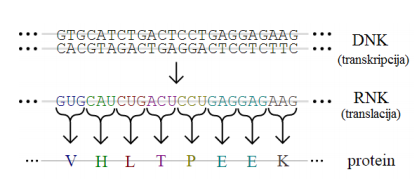
\includegraphics[width=0.5\textwidth]{Figures/BO/dogma.png}
    \caption{Prikaz centralne dogme molekularne biologije~\cite{JKd}}
    \label{fig:dogma}
\end{figure}

\subsection{Funkcije i osobine proteina}
Proteini su biološki najaktivniji molekuli sa velikim brojem esencijalnih uloga koje se dele na:
\begin{itemize}
\item dinamičke, od kojih su najvažnije:
\begin{enumerate} 
\item transportna - prenos molekula (poput kiseonika, gvožđa, lipida) i hormona od mesta sinteze do mesta delovanja,
\item biološka - regulacija metaboličkih procesa u ćeliji, kontrola i regulacija transkripcije gena i translacija,
\item katalizatorska - biološka katalizacija \footnote{Katalizacija predstavlja proces povećavanja brzina reakcija},
\item zaštitna - keratin, koagulacija krvi,
\item održavanje zapremine tečnosti u organizmu,
\end{enumerate}
\item strukturne, od kojih su najvažnije:
\begin{enumerate}
\item obezbeđivanje čvrstine i elastičnosti organa,
\item davanje oblika organizmu,
\item izgradnja strukturnih elemenata ćelije i
\item bitna uloga u kontraktilnim i pokretnim elementima organizma~\cite{spasic}.
\end{enumerate}
\end{itemize} 

Postoji nekoliko osobina koje karakterišu proteine, to su:
\begin{itemize}
\item izgradnja kompleksnih jedinjenja sa različitim supstancama po principu strukturne komplementarnosti i  
\item visoka osetljivost na različite agense koji ih denaturišu \footnote{Denaturacija proteina je proces koji izaziva promene u strukturi proteina menjajući i njihovo fiziološko dejstvo.}. Neki od agenasa su: visoka temperatura, pritisak, mehaničko tretiranje, dejstvo kiselina, baza, organskih rastvarača, materija, itd.~\cite{spasic}.
\end{itemize}
 
\subsection{Struktura proteina}
Struktura proteina zavisi od rasporeda aminokiselina i utiče na njegovu funkciju. Niska aminokiselina sadrži sve potrebne informacije kako bi se formirala trodimenzionalna struktura proteina, za koju se smatra da je najstabilnija~\cite{biopathways}. Ona se formira presavijanjem polipeptidnog lanca na različite načine. Unutrašnjost takve strukture ima visoku gustinu, pa takav lanac ne dopušta promene u sastavu i zahteva prisustvo aminokiselina tačno određene veličine~\cite{spasic}.
Uobičajena raspodela aminokiselina u proteinima je daleko od ravnomerne. Neke aminokiseline se javljaju mnogo češće od ostalih, tako se, na primer, leucin pojavljuje devet puta više od triptofana~\cite{biopathways}. \\\\
Proteinsku strukturu održavaju različite vrste kovalentnih i nekovalentnih interakcija između hemijskih skupina, npr. vodonične, jonske, elektrostatičke, dipolne, itd.. Nabiranjem i uvijanjem lanaca nastaju različiti oblici proteina: vlaknasti, globularni ili eliptični~\cite{medbio}.
Ako mutacija dovede do toga da aminokiselina sa malim bočnim lancem bude zamenjena aminokiselinom sa velikim, pojaviće se problem sa formiranjem trodimenzionalne strukture. Ako bi se, pak, velika aminokiselina zamenila sa malom, pojavio bi se prazan prostor, što bi moglo dovesti do destabilizacije molekula proteina~\cite{spasic}. \\\\
U molekulima proteina postoji hijerarhijska strukturalna organizacija u četiri nivoa:
\begin{enumerate}
\item primarna,
\item sekundarna,
\item tercijarna i
\item kvaternarna~\cite{spasic}.
\end{enumerate}
Na slici \ref{fig:structures} se može videti opšti prikaz mogućih struktura proteina, a na drugoj \ref{fig:structures2} šematski prikaz.
\begin{figure}[h]
	\centering
    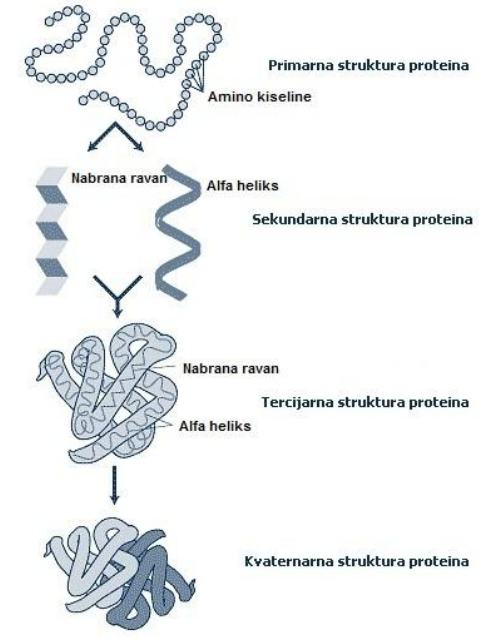
\includegraphics[width=0.5\textwidth]{Figures/BO/protein_structures.png}
    \caption{Prikaz struktura proteina}
    \label{fig:structures}
\end{figure}
\begin{figure}[h]
	\centering
    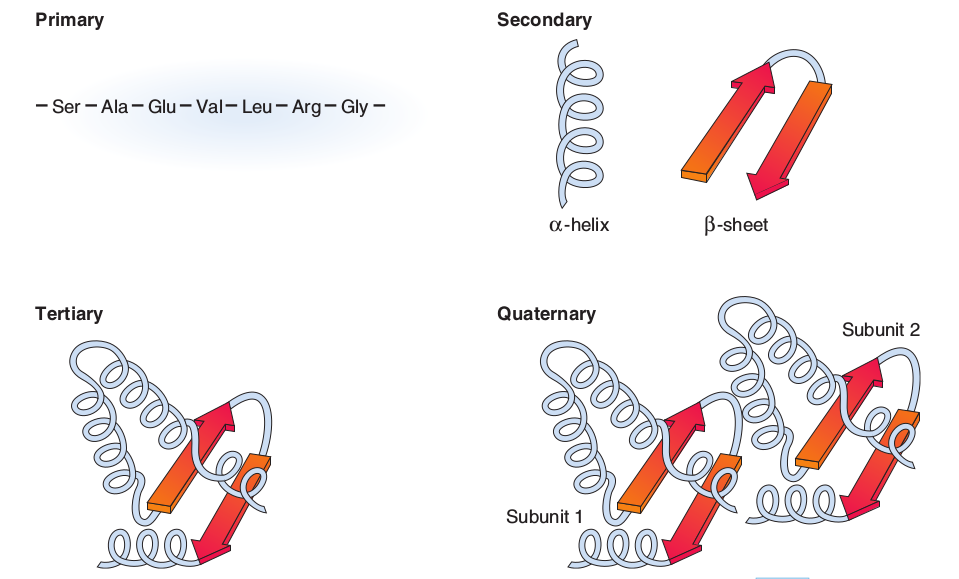
\includegraphics[width=1\textwidth]{Figures/BO/structure_schema.png}
    \caption{Šematski prikaz struktura proteina~\cite{bmbg}}
    \label{fig:structures2}
\end{figure}
\subparagraph{Primarna struktura}
Predstavlja s\^amu sekvencu aminokiselina\footnote{Redosled kojim su aminokiseline poređane u nekom polipeptidu se zove sekvenca aminokiselina~\cite{spasic}.} koje učestvuju u izgradnji proteina. Ona je od ključnog značaja za funkciju proteina zbog interakcija između bočnih lanaca aminokiselina koji određuju trodimenzionalnu strukturu. Proteini koji imaju sličnu sekvencu aminokiselina su $homologi$, a poređenje sekvenci među takvim proteinima može ukazati na genetsku relaciju između različitih vrsta~\cite{spasic}.\\\\
Mnoge genetske bolesti rezultuju u proteinima sa abnormalnim redosledom aminokiselina, što uzrokuje nepravilno presavijanje i gubitak ili nemogućnost normalnog funkcionisanja. Ukoliko su nam poznate strukture normalnih i mutiranih proteina, te informacije možemo iskoristiti za dijagnostikovanje ili proučavanje bolesti~\cite{lippincott}. Primarna struktura će sa mutacijama, u najmanju ruku, izmeniti unos, brisanje ili menjanje aminokiselina. Promene u primarnoj strukturi mogu imati uticaja i na više nivoe proteinskih struktura. Takve promene često dovode do lošeg presavijanja proteina i mogu dovesti do njegovog gubitka funkcije~\cite{flash}.
Prikaz izgleda primarne strukture na primeru insulina kod čoveka se vidi na slici \ref{fig:insulin}.
\begin{figure}[h]
	\centering
    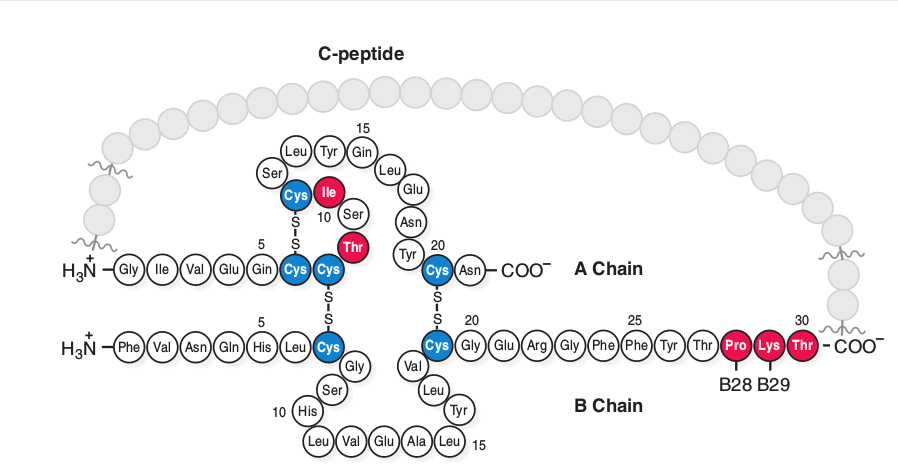
\includegraphics[width=1\textwidth]{Figures/BO/insulin.png}
    \caption{Prikaz primarne strukture~\cite{bmbg}}
    \label{fig:insulin}
\end{figure}
\subparagraph{Sekundarna struktura}
Odnosi se na oblik koji protein zauzima u prostoru i označava pravilno pojavljivanje ponavljanog prostornog rasporeda primarne strukture, u jednoj dimenziji~\cite{medbio}.
Ovu strukturu čini nekoliko različitih oblika, od kojih su najčešći $\alpha$-heliks i $\beta$-presavijena traka (ili $\beta$-struktura), a čest je i tzv. $\beta$-okret~\cite{spasic}.\\\\
\textbf{$\alpha$-heliks} - tip sekundarne strukture kod kog se gusto pakovani polipeptidni lanac spiralno uvrće. Karakteriše se brojem peptidnih jedinica po okretu i rastojanjem između dva okreta. Spada pod energetski najsiromašnije, a time, i najstabilnije strukture proteina. Heliks mogu obrazovati i $L-$ i $D-$ aminokiseline. Postoje dva tipa heliksa: levostrani i desnostrani~\cite{spasic}. Prikaz izgleda $\alpha$-heliksa se vidi na slici \ref{fig:aheliks}.
\begin{figure}[h]
	\centering
    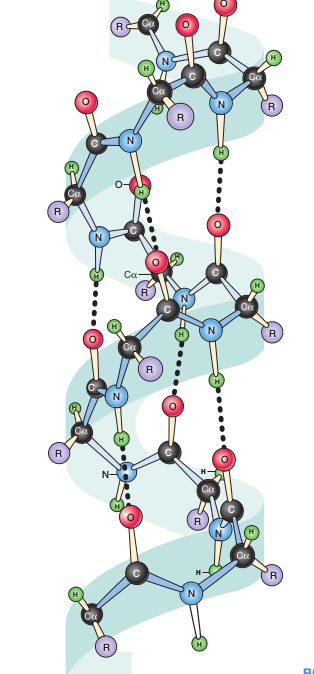
\includegraphics[width=0.25\textwidth]{Figures/BO/ahelix.png}
    \caption{Prikaz $\alpha$-heliksa~\cite{bmbg}}
    \label{fig:aheliks}
\end{figure}
 \\
\textbf{$\beta$-struktura} - Za razliku od $\alpha$-heliksa, sastoji se od dva ili više peptidnih lanaca, ili segmenata polipeptidnih lanaca, a obrazuje se kada se ovakvi tipovi lanca povežu uzdužno. Postoje dva tipa $\beta$-struktura: paralelna i antiparalelna~\cite{spasic}. Prikaz izgleda $\beta$-strukture se vidi na slici \ref{fig:beta}.\\

\begin{figure}[h]
	\centering
    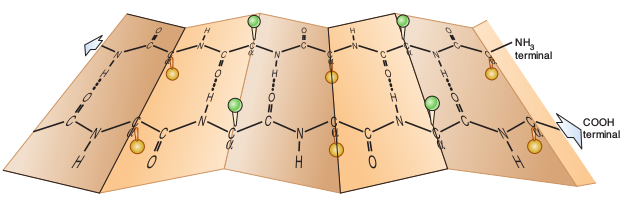
\includegraphics[width=1\textwidth]{Figures/BO/beta.png}
    \caption{Prikaz $\beta$-strukture~\cite{bmbg}}
    \label{fig:beta}
\end{figure}
\textbf{$\beta$-okreti} - obrću pravac polipeptidnog lanca praveći kompaktan globularan oblik~\cite{lippincott}. 
 
Prikaz izgleda sekundarnih struktura se nalazi na slici \ref{fig:ab}.
\begin{figure}[h]
	\centering
    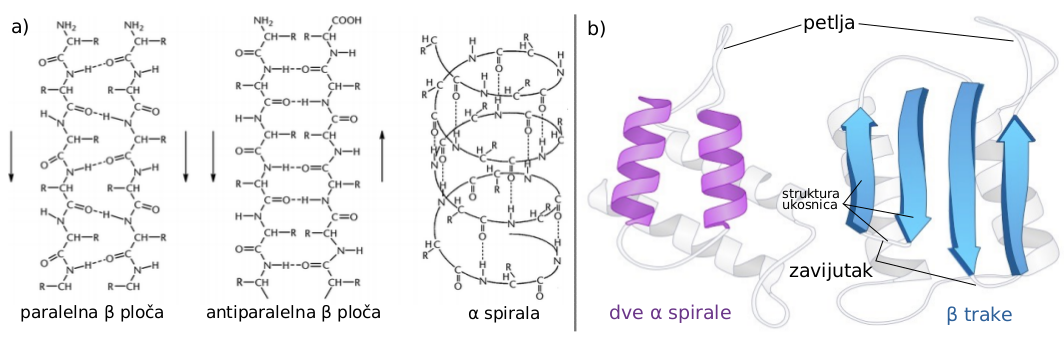
\includegraphics[width=1\textwidth]{Figures/BO/sec_structure.png}
    \caption{Prikaz sekundarnih struktura~\cite{Vinterhalter}}
    \label{fig:ab}
\end{figure}
 

\subparagraph{Tercijarna struktura}
Podrazumeva unutarmolekularno slaganje polipeptidnog lanca u kompaktnu trodimenzionalnu strukturu specifičnog oblika~\cite{medbio}.
Takva trodimenzionalna konformacija nastaje prostornim organizovanjem polipeptidnog lanca koji već ima sekundarnu strukturu. Na taj način se približavaju ostaci aminokiselina koji su udaljeni u primarnoj strukturi. Proteini koji imaju ovakvu strukturu su globularni i kompaktni sa velikom gustinom u središtu~\cite{spasic}.
\subparagraph{Kvaternarna struktura}
Predstavlja agregaciju više peptidnih lanaca u molekulu proteina~\cite{medbio}. Mnogi proteini, posebno oni velike mase, izgrađeni su od nekoliko polipeptidnih lanaca. Svaka takva komponenta naziva se $podjedinica$ ili $protomer$. Oni mogu biti identični\footnote{Tada takve proteine nazivamo $oligomerima$} ili se razlikovati prema strukturi. Ovakav raspored dovodi do brzog i efikasnog transfera substrata od jednog aktivnog centra enzima do drugog~\cite{spasic}.
 
\subsection{Savijanje proteina}
Interakcije između lanaca aminokiselina, koji se nalaze sa strane, određuju kako se dugački polipeptidni lanac presavija u trodimenzionalni oblik funkcionalnog proteina. Presavijanje proteina koje se događa u ćeliji traje od nekoliko sekundi do nekoliko minuta. 
Na slici \ref{fig:folding} se može videti opšti prikaz savijanja proteina.
\begin{figure}[h]
	\centering
    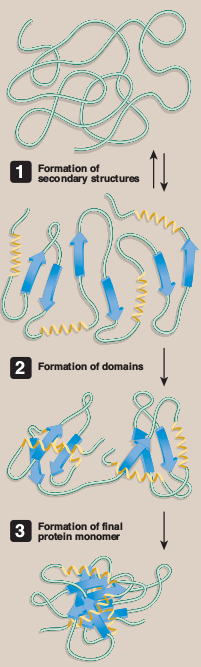
\includegraphics[width=0.25\textwidth]{Figures/BO/protein_folding.png}
    \caption{Prikaz savijanja proteina~\cite{lippincott}}
    \label{fig:folding}
\end{figure}

\subsection{Denaturacija proteina}
Denaturisanje proteina rezultuje u odvijanju i dezorganizaciji proteinske sekundarne i tercijarne strukture. Pod idealnim uslovima, denaturisanje proteina može biti $reverzibilno$. To znači da bi se protein, pri prestanku delovanja agenasa, vratio u normalno stanje. Međutim, većina proteina ostaje trajno neuređena~\cite{lippincott}. O neuređenosti proteina biće više reči u nastavku.\\\\
Jedno od objašnjenja zašto se protein ne vraća u originalno stanje se sastoji u tome da protein počinje sa savijanjem pre nego što se izvrši sinteza celog lanca. Osim toga, specijalizovana grupa pomoćnih proteina (engl. $chaperones$) je neophodna za pravilno savijanje mnogih vrsta proteina. Ovi pomoćni proteini interaguju sa polipeptidima u nekoliko faza tokom procesa savijanja, imaju ulogu u tome da održavaju protein nesavijenim dok sinteza nije gotova, ili imaju ulogu katalizatora. Loše savijanje proteina može dovesti do različitih bolesti kao što su: amiloidna bolest ili Prionova bolest~\cite{lippincott}.

% -------------------------------------------------------------------------------------------------
\section{Neuređenost proteina}
% -------------------------------------------------------------------------------------------------

Sa porastom broja proteina za koje je eksperimentalno utvrđena sekundarna struktura uočeno je da značajan broj proteina ne poseduje dobro definisanu, uređenu trodimenzionalnu strukturu, pod određenim fiziološkim uslovima. Usled velikog broja termina koji se koriste za opisivanje ovakvih proteina: prirodno/suštinski neuređeni, nesavijeni, denaturisani ili reomorfni proteini (eng.~{\em intrinsically disordered/ unfolded/ unstructured})~\cite{JKd}, u ovom radu, kao i u ~\cite{JKd}, biće korišćen samo kraći termin - neuređeni proteini. Neuređen može biti ceo protein, a mogu biti neuređeni određeni regioni proteina različitih dužina. \\\\
Neuređenost je inherentno\footnote{Inherentno = nasleđeno} svojstvo sekvence~\cite{IDP}. Statističkom analizom došlo se do zaključka da se aminokiseline mogu klasterovati na dve grupe: 
\begin{enumerate}
\item aminokiseline koje promovišu uređenost (eng.~{\em order promoting}) i
\item aminokiseline koje promovišu neuređenost (eng.~{\em disorder promoting})~\cite{Vinterhalter, IDPIDPr, DPC}.
\end{enumerate}

Veza koja postoji između sekvence i strukture ukazuje na to da je neuređenost enkodirana inherentna osobina~\cite{IDP}, odatle, naziv inherentno neuređeni proteini, skraćeno IDP\footnote{eng.~{\em Intrinsically Disordered Proteins}}, a ako su u pitanju neuređeni, ali funkcionalni, regioni, onda je skraćenica IDPr\footnote{eng.~{\em Intrinsically Disordered Protein Regions}}~\cite{Vinterhalter}.

Neuređene proteine ili neuređene regione je teško kategorizovati~\cite{IDP, IDPIDPr}, a jedan od opštih opisa strukture dat je kao kombinacija više tipova foldona\footnote{Foldon ostaje u originalnom nazivu, kao posledica manjka literature.~\cite{Vinterhalter}}:
\begin{itemize}
\item foldon (eng.~{\em foldon}) je nezavisno organizujuća jedinica(region) proteina,
\item indukativni foldon (eng.~{\em inducible foldon}) je neuređeni region proteina koji savijanje lanca postiže barem delom vezivajući se za partnera,
\item ne-foldon (eng.~{\em non-foldon}) je neuređeni region proteina koji nikada ne postiže uređenost,
\item polu-foldon (eng.~{\em semi-foldon}) je neuređeni region proteina koji ostaje polovično neuređen i nakon vezivanja za partnera, i 
\item anti-foldon (eng.~{\em unfoldon}) je region proteina koji iz uređenog prelazi u neuređeno stanje u cilju izvršavanja neke funkcije~\cite{Vinterhalter,DPC}.
\end{itemize}

Hipoteza proteinskog trojstva~\cite{IDP} govori o tome da funkcija proteina zavisi od bilo kog od tri moguća stanja (oblika) ili prelaza između tih stanja~\cite{Vinterhalter}. Svaki od narednih oblika može predstavljati prirodno stanje proteina i imati uticaja na njegovu ulogu u ćeliji. Neki proteini mogu prelaziti iz neuređenog u uređeno stanje, i obratno. Proteini se mogu pojavljivati u raznim oblicima:
\begin{enumerate}
\item uređen protein,
\item topljiva globula (eng.~{\em molten globule}),
\item pre-topljiva globula (eng.~{\em pre-molten globule}) i 
\item nasumično klupko (eng.~{\em random coil})~\cite{Vinterhalter, JKd}.
\end{enumerate}


Neuređenost proteina se utvrđuje eksperimentalno, laboratorijskim analizama, ili uz pomoć prediktora za automatsko utvrđivanje neuređenosti. 

\subsection{Eksperimentalno ispitivanje neuređenosti proteina}

Eksperimentalno utvrđivanje neuređenosti proteina podrazumeva laboratorijsko, eksperimentalno, utvrđivanje neuređenosti korišćenjem raznih biofizičkih i biohemijskih tehnika i njihovih kombinacija. Ono spada u veoma skupe, spore i metode koje ne mogu da odgovore na izazove akademije i industrije. Uprkos tome, razvijen je veliki broj metoda za karakterizaciju strukture i osobina proteina. Svaka eksperimentalna metoda karakteriše se raznim prednostima manama i nivoom pouzdanosti metode, zbog čega je najbolje ovakve metode kombinovati. Naredne eksperimentalne, biofizičke i biohemijske, tehnike su najčešće u ispitivanju neuređenosti proteina~\cite{IDP,JKd}:
\begin{itemize}
\item Kristalografija X-zracima(eng.~{\em X-ray crystallography}),
\item Spektroskopija Nuklearnom Magnetnom Rezonancom (eng.~{\em NMR spectroscopy}),
\item Cirkularni dihroizam (eng.~{\em Circular dichroism (CD) spectroscopy}),
\item Senzitivnos na proteolizu (eng.~{\em Sensitivity to proteolysis}),
\item Ramanova optička aktivnost, itd. 
\end{itemize}

\subsection{Računarsko ispitivanje neuređenosti proteina}

Kao posledica osobina eksperimentalnog ispitivanja neuređenosti, veliki napori su uloženi u razvoj prediktora za računarsko utvrđivanje neuređenosti proteina. Ovi prediktori uz pomoć računara, korišćenjem tehnike mašinskog učenja, vrše utvrđivanje neuređenosti proteina. Iz godine u godinu, broj ovih prediktora je sve veći, a u zadnje vreme se radi i na kreiranju metaprediktora, koji predviđanje vrše kombinovanjem više tehnika. O ovoj vrsti predikcije biće više reči u narednom poglavlju.\\\\

% Chapter Template

\chapter{Predikcija neuređenosti proteina} % Main chapter title
\label{predikcija} % Change X to a consecutive number; for referencing this chapter elsewhere, use \ref{ChapterX}

Razvitak istraživanja o neuređenim proteinima počinje oko 1978. godine, kada sa razvojem kristalografije X-zracima i spektroskopije nuklearnom magnetnom rezonancom, uspešno ukazuje na funkcionalne poremećaje u proteinima, čime istraživanje dobija na značaju. Tokom prvih godina, pojavljuju se mnogobrojni nazivi $"$osetljivi$"$,$"$reomorfični$"$,$"$mobilni$"$,$"$kameleonski$"$,$"$igrajući$"$ i drugi. Usled velikog broja termina koji se, i kasnije, koriste za opisivanje ovakvih proteina: prirodno/suštinski neuređeni, nesavijeni, denaturisani ili reomorfni proteini (eng.~{\em intrinsically disordered/ unfolded/ unstructured}), u ovom radu, biće korišćen samo kraći termin - neuređeni proteini. 
Neuređeni proteini bitnu ulogu u određivanju ćelijskog odgovora na spoljašnje uticaje, transkripciju i translaciju, kao i savijanje i odvijanje ćelijskih makromolekula.
Kao što je navedeno u prethodnom poglavlju, neuređenost proteina se može, osim eksperimentalnog, određivati i računarski. Upravo o tom vidu određivanja, odnosno, predikcije, neuređenosti proteina govori ovo poglavlje. Najpre, biće detaljnije opisan računarski postupak. Nakon toga, biće priče o prediktorima, od kojih će pojedini biti detaljnije objašnjeni. Na kraju, ukratko, će biti predstavljena baza podataka DisProt i njen značaj u ovom radu.~\cite{IDPsAtoZ,JKd, IDPTompa}\\\\
Značaj pronalaska neuređenih proteina/regiona leži, pre svega, u tome što uočavanjem ovakvih regiona poboljšavamo analizu proteina i time izbegavamo poravnavanje uređenih i neuređenih proteinskih regiona čime se povećava preciznost analize sličnosti sekvenci. Još jedan bitan razlog je ušteda vremena pri upotrebi eksperimentalnih tehnika, jer dolazi do velikih gubitaka vremena na utvrđivanje strukture proteina koji je nema.~\cite{POverview, COverview} 

%----------------------------------------------------------------------------------------
%	SECTION 1
%----------------------------------------------------------------------------------------

\section{Prediktori}

Više od sedamdeset prediktora razvijeno je od $1997.$ godine, od čega čak sedamnaest u periodu između $2010.$ i $2014.$. Ovi prediktori se mogu ugrubo podeliti u nekoliko kategorija, one bazirane na~\cite{PredictorsOverview}:
\begin{enumerate}
\item klasifikatorima mašinskog učenja,
\item meta-pristupu (kombinovanjem predikcija više prediktora) i 
\item fizičko-hemijskim karakteristikama.
\end{enumerate}

Svaki prediktor koristi različite koncepte, fizičko-hemijske karakteristike ili različite algoritme mašinskog učenja. Međutim, ni ove metode nisu najpouzdanije. Postoje dva glavna izvora nepouzdanosti predikcije neuređenosti koji dolaze iz:
\begin{itemize}
\item nepouzdanosti modela i
\item nepouzdanosti podataka.
\end{itemize}

Pouzdanost (ili nepouzdanost) modela zavisi od odabranog modela. Odabir modela se vrši tako što iz skupa dostupnih modela bira onaj čija je preciznost veća u odnosu na ostale dostupne modele, testiranjem na zadatom skupu sekvenci.
Nepouzdanost podataka se odnosi na  ~\cite{MolBioSyst}


%-----------------------------------
%	SUBSECTION 1
%-----------------------------------
\subsection{SPOT-D}

SPOT-Disorder Predictor je razvijen da ima visoku efikasnost u predviđanju i kratkih i dugih neuređenih regiona bez odvojenog treninga, bez obrzira na činjenicu da neuređeni regioni različitih veličina imaju različite sastave aminokiselina. SPOT-D je metod koji je nastao unapređivanjem metoda koji koristi tradicionalne neuralne mreže bazirane na prozorima nad svim testiranim skupovima bez odvajanja trening skupa na kratkim i dugim regionima. Utvrđeno je da je SPOT-D jednako ili više precizan u odnosu na ostale metode. Ovaj metod oslikava prednosti kombinovanja LSTM (eng. Long Short Term Memory) neuronskih mreža sa dubokim dvosmernim rekurentnim neuronskim mrežama, kako bi se uočile interakcije između proteina.
~\cite{SPOTD}


%-----------------------------------
%	SUBSECTION 2
%-----------------------------------

\subsection{PONDR}
PONDR prediktor vrši predikciju nad pojedinačnim sekvencama korišćenjem neuronskih mreža sa propagacijom unapred (eng. feedforward neural networks) koje koriste sekvence atributa nad prozorima od $9$ do $21$ aminokiseline. Uzima se prosek nad ovim prozorima, a potom se te vrednosti koriste pri treniranju neuronskih mreža tokom konstrukcije prediktora. Iste vrednosti se koriste za ulaze da bi se napravila predikcija. Prediktori neuronskih mreža se treniraju nad neponavljajućim skupovima uređenih i neuređenih sekvenci,a izlazi su brojevi između $0$ i $1$, koji se odvajaju na prozore od po $9$ aminokiselina. Ako vrednost regiona prevazilazi prag od $0.5$ smatra se da je region neuređen.


%-----------------------------------
%	SUBSECTION 3
%-----------------------------------

\subsection{s2D}


%-----------------------------------
%	SUBSECTION 4
%-----------------------------------

\subsection{IUPred}
IUPred vrši previđanje neuređenosti proteina sa loše definisanom tercijarnom strukturom (eng. Intrinsically unstructured/disordered proteins - IUPs) na osnovu sekvenci aminokiselina procenjujući njihovu energiju prilikom interakcija. Metod se bazira na fizičkim osnovama uređene/neuređene prirode proteina. Naime, globularni proteini prave veliki broj interakcija, čime se obezbeđuje stabilizujuća energija koja nadoknađuje određene gubitke prilikom savijanja proteina. Nasuprot njima, neuređeni proteini imaju specijalne regione koji nemaju sposobnost kreiranja interakcija.\\\\

Pristup korišćen pri razvoju ovog prediktora se zasniva na statističkoj proceni mogućnosti polipeptida da formiraju takve stabilne veze (interakcije). Pretpostavka koja postoji je da se neuređene sekvence ne savijaju zbog nemogućnosti da ostvare dovoljno stabilne veze prilikom interakcija. Pokazalo se da je suma energije prilikom interakcija može da se proceni matematički na osnovu sastava aminokiselina, uzimajući u obzir da doprinos aminokiselina uređenosti zavisi od hemijskog tipa aminokiseline i njene sposobnosti da interaguje sa drugima. Prilikom predikcije, mogu se koristiti ugrađeni parametri koji su optimizovani za predviđanje kratkih ili dugačkih neuređenih regiona. ~\cite{IUPred, IUPred1, IUPred2, IUPred3}


%-----------------------------------
%	SUBSECTION 5
%-----------------------------------
 
\subsection{ESpritz}
ESpritz detektuje neuređene regione primarne strukture i bazira se na efikasnom sistemu za predviđanje koji ih pronalazi. Određivanje neuređenosti iz niza aminokiselina je težak problem, ali ova metoda daje obećavajuće rezultate. Postoje dva razloga za to:
\begin{itemize}
\item  ako niz aminokiselina određuje strukturu onda nestrukturirani regioni aminokiselina mogu imati drugačije osobine, 
\item neuređenost je bitna za mnogobrojne biološke funkcije, pa je prisutna očuvanost neuređenih proteina tokom evolucije. 
\end{itemize}

ESpritz, pri svom radu, koristi dvosmerne rekurentne neuronske mreže (engl. BRNN - Bidirectional recursive neural network) i treniran je na više različitih tipova neuređenosti. Algoritam uči kontekst informacija kroz rekurzivnu dinamiku mreže, smanjujući time broj parametara i implicitno izvlačeći informacije iz sekvence. Ovo je efikasan metod za pojedinačne sekvence i bazira se na sekvenci, bez korišćenja skupih izračunavanja kako bi pronašao poravnanja više sekvenci. Tipovi predviđanja neuređenosti nad kojima je ESpritz treniran su:
\begin{itemize}
\item Kratki x-zraci (eng. short x-ray): bazirano na nedostajućim atomima u strukturama koje su rešene sa X-zracima i nalaze se u PDB-a (eng. PDB - Protein Data Bank), ovaj tip predviđanja koristi se kod kraćih proteina. 
\item Duži disprot: skup podataka koji se koristi za ovaj tip sadrži duže neuređene segmente u odnosu na prethodni tip. Bazira se na funkcionalnim atributima neuređenih regiona. Smatra se da je pronađen neuređeni region ako se utvrdilo barem jednom da je neki region neuređen. Svi ostali regioni se smatraju uređenim.
\item NMR pokretljivost.
\end{itemize}
ESpritz određuje verovatnoću poremećaja za svaki region. ~\cite{ESpritzAFPD, ESpritzEP, ESpritz2, ESpritz3}


%-----------------------------------
%	SUBSECTION 6
%-----------------------------------

\subsection{SEG}


%-----------------------------------
%	SUBSECTION 7
%-----------------------------------

\subsection{Disopred2}

%----------------------------------------------------------------------------------------
%	SECTION 2
%----------------------------------------------------------------------------------------

\section{Baza podataka DisProt}

% =================================================================================================
\chapter{Aplikacija}
% =================================================================================================

% -------------------------------------------------------------------------------------------------
\section{Arhitektura}
% -------------------------------------------------------------------------------------------------

% -------------------------------------------------------------------------------------------------
\section{Funkcionalnosti}
% -------------------------------------------------------------------------------------------------

\section{Korišćenje aplikacije}
% -------------------------------------------------------------------------------------------------

\section{Primer upotrebe}
% -------------------------------------------------------------------------------------------------

% =================================================================================================
\chapter{Zaključak}
% =================================================================================================
Aplikacija kreirana ovim radom omogućava korisniku da na veoma jednostavan način dobije pregled neuređenih regiona proteina kroz jasan i nedvosmislen interfejs. Najveći doprinos ovog rada leži u tome što objedinjuje odluke više prediktora i stavlja ih praktično pod okrilje jedne aplikacije, čime se ističu jednostavnost i pouzdanost, izražena metrikama, pri donošenju odluka. Moguća unapređenja rada leže u parametrizaciji prediktora, povećanju njihove brojnosti, kao i u dodeljivanju težina prediktorima. 

% 
\chapter{Implementacija} % Main chapter title

\label{Implementacija} % For referencing 


%------------------------------------------------------------------------------





%\include{Chapters/Rezultati}

%----------------------------------------------------------------------------------------
%	THESIS CONTENT - APPENDICES
%----------------------------------------------------------------------------------------

\appendix % Cue to tell LaTeX that the following "chapters" are Appendices

% Include the appendices of the thesis as separate files from the Appendices folder
% Uncomment the lines as you write the Appendices

% % Appendix A

\chapter{Frequently Asked Questions} % Main appendix title

\label{AppendixA} % For referencing this appendix elsewhere, use \ref{AppendixA}

\section{How do I change the colors of links?}

The color of links can be changed to your liking using:

{\small\verb!\hypersetup{urlcolor=red}!}, or

{\small\verb!\hypersetup{citecolor=green}!}, or

{\small\verb!\hypersetup{allcolor=blue}!}.

\noindent If you want to completely hide the links, you can use:

{\small\verb!\hypersetup{allcolors=.}!}, or even better: 

{\small\verb!\hypersetup{hidelinks}!}.

\noindent If you want to have obvious links in the PDF but not the printed text, use:

{\small\verb!\hypersetup{colorlinks=false}!}.

%\include{Appendices/AppendixB}
%\include{Appendices/AppendixC}

%----------------------------------------------------------------------------------------
%	BIBLIOGRAPHY
%----------------------------------------------------------------------------------------
\renewcommand{\bibname}{Bibliografija}
\printbibliography[heading=bibintoc]

%----------------------------------------------------------------------------------------

\end{document}  
